% Typeset with XeTeX
% Allows use of system fonts rather than just LaTeX's ones
% NOTE - if you use TeXShop and Bibdesk (Mac), can complete citations
%  - open your .bib file, type~\citep{xx... and then F5 or Option-Escape
\documentclass[11pt]{article}
\usepackage[margin=1in, letterpaper]{geometry} % set page layout
%\geometry{letterpaper}  % or a4paper
\usepackage[xetex]{graphicx} % allows us to manipulate graphics.
% Replace option [] with pdftex if you don't use Xe(La)TeX
\usepackage{color}
\usepackage{indentfirst}
\usepackage{hyphenat}
\usepackage{epstopdf} % automatic conversion of eps to pdf 
\usepackage{amsmath, amssymb} % Better maths support & more symbols
\usepackage{textcomp} % provide lots of new symbols - see textcomp.pdf
% line spacing: \doublespacing, \onehalfspacing, \singlespacing
\usepackage{setspace}

\singlespacing
\usepackage{pgfplotstable}
% allows text flowing around figs
% use \begin{wrapfigure}{x}{width} where x = r(ight) or l(eft)
\usepackage{wrapfig}
\usepackage[parfill]{parskip} % don't indent new paragraphs
\usepackage{flafter}  % Don't place figs & tables before their definition 
\usepackage{verbatim} % allows \begin and \end{comment} regions
\usepackage{booktabs} % makes tables look good
\usepackage{bm}  % Define \bm{} to use bold math fonts
% linenumbers in L margin, start & end with \linenumbers \nolinenumbers,
\usepackage{lineno} % use option [modulo] for steps of 5
\usepackage[auth-sc]{authblk} % authors & institutions - see authblk.pdf
%\renewcommand\Authands{ and } % separates the last 2 authors in the list
% control how captions look; here, use small font and indent both margins by 20pt
%{\usepackage[font={sf, footnotesize}]{caption} 

\usepackage[margin=10pt,font={footnotesize,sf}, labelfont=bf, labelsep=endash]{caption}

\setlength{\captionmargin}{20pt}

%: FONT
% If you don't want to use system fonts, replace from here to 'Citation style' with \usepackage{Palatino} or similar
%: ************ FANCY FONTS START HERE
\usepackage[no-math]{fontspec} % 'no-math' = keep computer modern for math fonts
\usepackage{xunicode} % needed by XeTeX for handling all the system fonts nicely
\usepackage[no-sscript]{xltxtra} 
\setmonofont[Scale=0.8]{PT Serif} % typeface for \tt commands
\setsansfont{Avenir} 
\defaultfontfeatures{Mapping=tex-text}
\setmainfont{Minion Pro}
%\setmainfont{Source Sans Pro}
%: ************ FANCY FONTS END HERE

%:CITATION STYLE
% natbib package: square,curly, angle(brackets)
% colon (default), comma (to separate multiple citations)
% authoryear (default),numbers (citations style)
% super (for superscripted numerical citations, as in Nature)
% sort (orders multiple cites into order of appearance in ref list, or year if authoryear)
% sort&compress: as sort, + multiple citations compressed (as 3-6, 15)
\usepackage[numbers,comma,sort&compress]{natbib}
\usepackage{nicefrac}
\usepackage{multirow}

%:SHORTCUT COMMANDS
% Maths
\newcommand{\ddt}[1]{\ensuremath{\frac{{\rm d}#1}{{\rm d}t}}}  % d/dt
\newcommand{\dd}[2]{\ensuremath{\frac{{\rm d}#1}{{\rm d}#2}}} % dy by dx  - \dd{y}{x}
\newcommand{\ddsq}[2]{\ensuremath{\frac{{\rm d}^2#1}{{\rm d}#2^2}}} % second deriv
\newcommand{\pp}[2]{\ensuremath{\frac{\partial #1}{\partial #2}}} % partial \pp{y}{x}
\newcommand{\ppsq}[2]{\ensuremath{\frac{\partial^2 #1}{\partial {#2}^2}}}
\newcommand{\superscript}[1]{\ensuremath{^{\textrm{#1}}}} %normal (non-math) font for super/subscripts in text
\newcommand{\subscript}[1]{\ensuremath{_{\textrm{#1}}}}
\newcommand{\positive}{\ensuremath{^+}}
\newcommand{\negative}{\ensuremath{^-}}
% Editing
\newcommand{\red}[1]{{\color{red}{#1}}}
\newcommand{\redtext}[1]{{\color{red}{#1}}}
\newcommand{\blue}[1]{{\color{blue}{#1}}}
\newcommand{\bluetext}[1]{{\color{blue}{#1}}}
\newcommand{\scinot}[2]{\ensuremath{#1 \times 10^{#2}}}
% Standard stuff
\newcommand{\be}{\begin{equation}}
\newcommand{\ee}{\end{equation}}
\newcommand{\bea}{\begin{eqnarray}}
\newcommand{\eea}{\end{eqnarray}}
\newcommand{\ie}{\textit{i.e.}}
\newcommand{\etal}{\textit{et al.}}
\newcommand{\khi}{Ki67$^\text{hi}$}
\newcommand{\klo}{Ki67$^\text{lo}$}
\newcommand{\looic}{$\Delta$LOO-IC}

% \begin{graybox} text \end{graybox} for text with a background colour
\definecolor{MyGray}{rgb}{0.96,0.97,0.98}
\definecolor{MyGray}{rgb}{0.96,0.90,0.98}
\makeatletter\newenvironment{graybox}{%
	\begin{lrbox}
		{\@tempboxa}\begin{minipage}[r]{0.98\columnwidth}}{\end{minipage}\end{lrbox}%
	\colorbox{MyGray}{\usebox{\@tempboxa}}
}\makeatother


%%%%%%%%%%%%%%%%%%%%%%%

\title{Population dynamics of  Follicular mature and germinal center B cells}
\author{}

\date{}

\begin{document} 
	\maketitle
	
	We aimed to quantify the dynamics of various subsets within mature B cell population and to understand the rules of replacement of old cells by that of new ones within each subset.
	%We adopted the conventional view of B cell development and assumed that Transitional 2 (T2) cells are the direct precursor of FM cells, which then participate in germinal centre (GC) reactions upon antigen interaction.
	
	%We define turnover to mean loss. 
	
	% In the busulfan chimeras, if the source is constant in time and all cells behave the same way, the existing population is replaced at rate $\lambda$, the net loss rate (turnover rate - division rate). 
	
	%So rate of replacement is not necessarily the rate of turnover (unless there is no division). Division compensates for turnover and keeps host cells in the pool for longer.
	
	%Might be worth coming up with a word for $\lambda$. I think 'clonal persistence --- low $\lambda$ means that a cell and its progeny survive for a long time (if $\lambda=0$, a clone persists for ever even though it may be dividing and dying; if $\lambda>0$, mean lifetime of a lineage (e.g. a cell and all its descendents) is $1/\lambda$. If $\lambda>0$, the cell population grows exponentially as $e^{\lambda t}$. 
	
	
	%\red{One concern: Sanket tried T1 as source and it actually gives better fits in all FM cases ({\looic} $\simeq$ 5). But we are going with dogma and saying T2 is source. It's puzzling to us that there is apparently so much residual Ki67 expression in FM from the T2 source, if all the division is pre-T1 as you say. Makes me worry a littl...} 
	
The busulfan chimera system allows us to follow the fate of newly made B cells as they develop and differentiate into mature B cell subsets. The kinetics with which new (donor-derived) B cells percolate into peripheral B cell subsets and displace older host-derived cels allow us to map their differentiation pathways, quantify their homeostatic dynamics, and determine the rules of replacement within each subset.
	
To help constrain the model fitting and parameter estimation,  we used observations from  Ki67-CreER-YFP reporter mice to put  priors on the net rates of loss of FM and GC B cells in spleen and LN. We measured  the frequencies of YFP-expressing cells  in these subsets  15 and 66d after the transient induction of YFP expression in cells expressing Ki67 \red{(Figure)}. Given that the compartments may also accumulate YFP+ from their upstream precursor populations during this period,  the decline in YFP expression each subset  yields approximate upper bounds on the net rate of loss of cells in each compartment \red{put these numbers on the YFP figure}.
	
	
\subsection*{Follicular Mature B cells are a homogeneous, slowly dividing population whose lifespan increases with age}

We generated timecourses of numbers and Ki67 expression levels of host and donor cells within the FM B cell pool in mice after the establishment of stable bone marrow chimerism in mice. To allow us to examine any impact of age on homeostatic dynamics, we generated chimerism in mice of ages spanning ?? and ??? weeks, and followed them out to a year of age. 	We wanted to use this information to	 assess the relative support for a variety of different models of FM B cell homeostasis, shown schematically in Figure~\ref{fig:FM-model-sketches}. We assumed that FM cells circulate freely in the lymphatic system \red{CITE} , and so we pooled the numbers of these cells recovered from spleen and lymph nodes when modelling their dynamics.
%	We compared different models of the population dynamics and structure of the FM compartment, as well as the possibilities that  the T1 or T2 transitional subsets are the immediate precursors of FM cells.
	%In order to compare the time-varying chimerism in FM cells across animals with different levels of bone marrow chimerism and different sources, we normalised the FM chimerism to that in the common progenitor population,  \ie T1 cells.
	%Here, we assess the suitability of T1, T2 and pooled (T1+T2) compartments as putative source populations for FM cells and explore various mechanisms that can explain their population dynamics in mice.
%	\subsection*{Replacement kinetics are consistent with FM cells being a single, kinetically homogeneous population, with cell lifetime increasing with host age}
%	The chimerism within the FM compartment stabilised at the level of the upstream transitional T1 population by about 210d post-BMT, implying the near-complete replacement of the compartment within that timeframe. Complete replacement suggests that the average rates of loss across host and donor cell populations are always equal. Additionally, we measured the expression of Ki67 in host and donor cells. Ki67 is a nuclear protein expressed during cell cycle and lost with a lifetime of a few days following mitosis (Gossel eLife 2017 \red{and others - see refs in that paper}). Immediately following BMT the donor FM cells are highly enriched for recently divided cells, with around 80\% \khi, but this proportion falls slowly to equalise with that of host cells at around 10\% after approximately 100 days. The kinetics of the size, donor chimerism and Ki67 expression  following bone marrow transplant are rich in information regarding the processes of division and turnover within the FM B cell pool. 
	%We assumed a mean lifetime of Ki67 post-mitosis of 3.5d, and also assumed that \khi\ and \klo\ cells are lost at equal rates $\delta(t)$. The timecourses of host and donor \khi\ fractions were then generated by simulating the model with its best-fit parameters, beginning at the mean \khi\ fractions observed at 12d post-BMT, pooled across all experimental cohorts. See Methods below for details.}

	

	
In all models we assumed that cells differentiate into FM B cells at a rate proportional to the size of their precursor population, which assumed could be either T1, T2, or T1 and T2 combined. The simplest model (Figure~\ref{fig:FM-model-sketches}A)  assumed that  FM B cells, whether host or donor, form a homogeneous population in which all cells are lost through death or differentiation  at the same rate $\delta$ and self-renew through division  at the same rate $\rho$. However the approach to stable chimerism appeared to initially be rapid and then gradually slow (Figure~\ref{fig:results_FM}B). To detect and describe any multiphasic behaviour we considered three extensions to this basic model. In the first, the rate of turnover ($\delta$) or division ($\rho$) might vary with host age (the `time dependent' model, Figure~\ref{fig:FM-model-sketches}B). In the second, FM B cells comprise two independent subpopulations turning over at different rates (Figure~\ref{fig:FM-model-sketches}C). In this we would expect the donor chimerism initially to increase rapidly as the subpopulation with faster turnover is replaced, followed by a more gradual approach to stable chimerism as the more persistent subpopulation, with slower turnover, is replaced. Third, we considered a model in which the FM pool is homogeneous with constant rates of division and turnover, but fed from the source population at a rate that declines with age  (Figure~\ref{fig:FM-model-sketches}D), which may also explain any decelerating approach to stable chimerism.  

	\begin{figure}[htbp] %  figure placement: here, top, bottom, or page
	   \centering
	   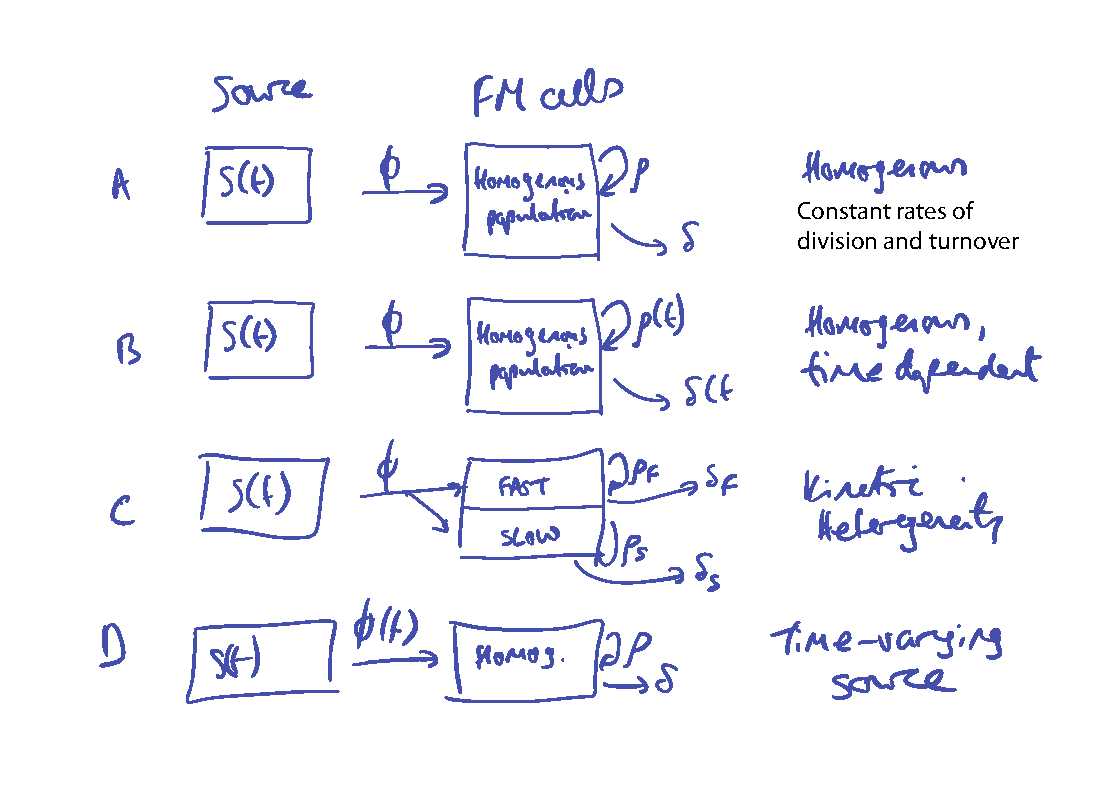
\includegraphics[width=0.8\linewidth]{figures/FM-Model-Sketches.pdf} 
	   \caption{Schematic descriptions of the candidate models of FM B cell homeostasis}
	   \label{fig:FM-model-sketches}
	\end{figure}
	
%\red{I think should drop incumbent. No signal in data to support trying it?}
%An alternative explanation of this time-varying kinetic is that the FM pool comprises independent sub-populations with different but constant rates of division and turnover, each fed from the T1 source.  In this scenario, less persistent populations (those with a high net loss rate $\lambda$) will be replaced most rapidly after BMT, giving an initial steep upslope in chimerism. There will then follow a slower increase as the more persistent FM subpopulations (with low $\lambda$) are replaced by donor cells relatively slowly.
We fitted each model  simultaneously to the timecourses of the total size of the FM pool, the chimerism within FM B cells normalised to that in T1 (the earliest common precursor to all populations considered), and the proportions of host and donor FM cells expressing Ki67. We found strongest support for the model in which the loss or turnover rate $\delta$ changes with host age and the division rate $\rho$ remains constant, with T1 transitional cells as the direct precursor of FM B cells.  Fits and data are shown in Fig.~\ref{fig:results_FM}; see Methods for the mathematical formulation of the models and the fitting strategy.  The measures of relative support for this and the alternative models are given in Table~\ref{tab:FM-AICs}.

 	\begin{figure}[htbp]
		\centerline{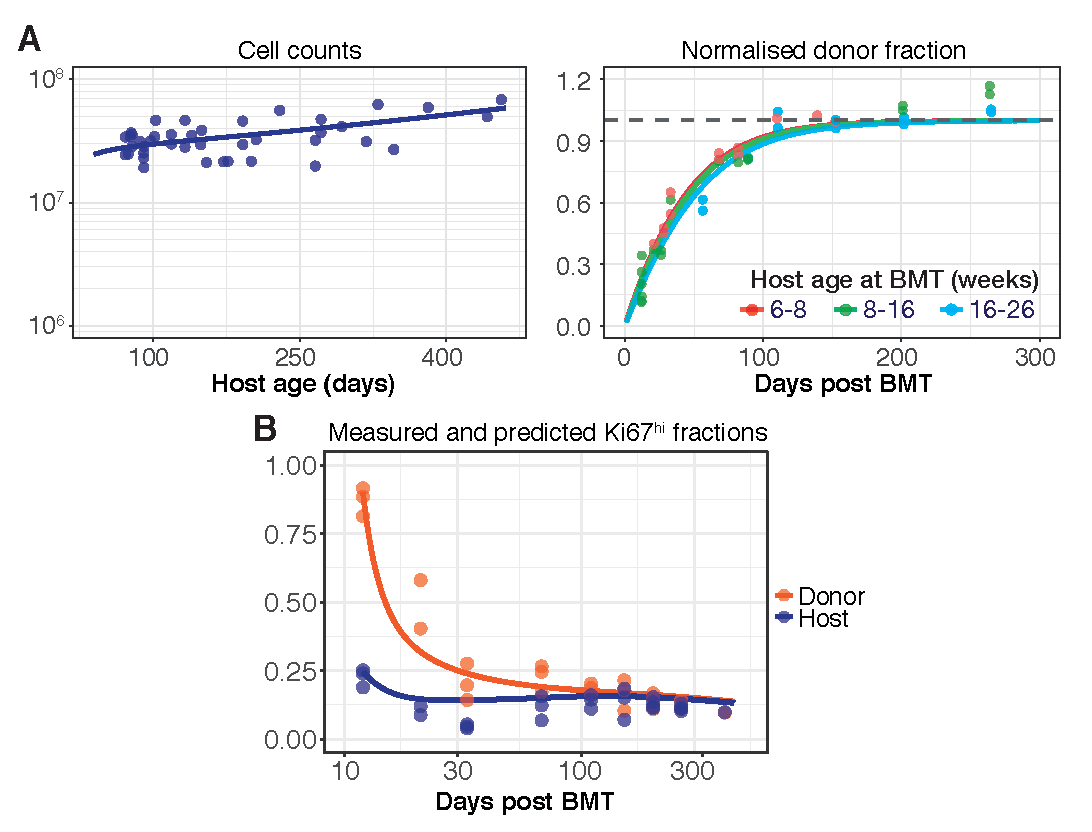
\includegraphics[scale = 0.85] {Results_FM.pdf}}
		\caption{ \textbf{Population dynamics of FM B cells in busulfan chimeric mice}, using the best-fitting model in which cells divide at a constant rate and their mean lifespan increases with host age.
		%The model was fitted simultaneously to the extended timecourses of total cell counts of FM B cells pooled from LN and spleen in busulfan chimeras, the donor fractions in FM B cells normalised to the chimerism in T1 cells and the proportion of cells that were \khi\ within host and donor FM B cells.
		Solid lines denote the most probable simultaneous description of the observations of (A) cell counts, (B) the  chimerism within FB cells normalised to that in T1,  and (C) the proportions of host and donor cells expressing Ki67. Shaded envelopes indicate the effect of uncertainty in parameters on the model fit, generated by drawing samples from the posterior distribution of parameter estimates and shading within the 4.5 and 95.5 percentiles of the resulting model predictions. Different colours in (A) and (B) indicate the model fits for mice grouped according to the age at which they underwent bone marrow transplant (BMT). Model predictions were generated using the mean age at BMT within each group.}
		\label{fig:results_FM}
	\end{figure}


 
  %This model of time-dependent loss was superior to the simplest model with constant rates of division and turnover ({\looic} = 8) and also superior to the alternative with a time-varying division rate (\looic = 10).

%: Table: FM model weights
	\begin{table}[htbp]
		\begin{center}
			\renewcommand{\arraystretch}{1.25}
			\begin{tabular}{c c c c c} 
				\toprule 
				\multicolumn{4}{c}{\textbf{Model and {\looic}}} \\
				\cline{2-5}
				Source &{\small Time-dependent}  & {\small Simple homogeneous} &  {\small Kinetic heterogeneity} & {\small Incumbent} \\ 
				\toprule
				T1      &   0             &              8             &                7              &          9         \\ 
				T2      &   36            &              43            &                39             &          42        \\ 
				T1 + T2 &   19            &              29            &                28             &          29        \\ 
				\hline
				\toprule 
			\end{tabular}
		\end{center}
		\caption{ \textbf{Comparison of models describing the population dynamics of Follicular Mature (FM) B cells}, pooled from LN and spleen. \red{switch to model weights, or add them} LOO-IC values obtained using leave-one-out cross validation method are shown relative to that of the best fitting model, in which the rate of loss  (turnover) of FM cells declines slowly with the age of the host. Predictions of more complex models were very close to those of the simple homogenous model (that is, either very little kinetic heterogeneity, close to zero incumbent cells, or effects of cells age on turnover or division rates)}. 
		\label{tab:FM-AICs}
	\end{table} 
	
	
We estimate that FM B cells  have a mean lifetime of roughly 34 days in 7 week-old mice, and that this life expectancy doubles on an average every 28 months. While levels of Ki67 in FM B cells are appreciable (approximately 10\%; Fig.~\ref{fig:results_FM}C), we find that the bulk of this derives from newly generated FM cells who inherit it from the highly proliferative T1 population; roughly 4\% of FM B cells are replaced each day by new immigrants and indeed the donor-derived FM B cells, which soon after BMT are highly enriched for newly generated cells, show significantly higher levels of Ki67 than host cells (Fig.~\ref{fig:results_FM}C).  We infer that FM B cells themselves self-renew infrequently, with an estimated mean interdivision time of approximately 9 months.  Because this self-renewal  is slow, the average lifetime of a clone (derived from the net rate of loss and proliferative renewal, $\delta-\rho$) is close to the life expectancy of individual cells. Parameter estimates and 95\% credible intervals are in Table~\ref{tab:FM-pars}.
	
	%: Table: FM parameter estimates
	\begin{table}[htbp]
		\begin{center}
			\renewcommand{\arraystretch}{1.25}
			\begin{tabular}{ l r l } 
				\toprule 
				\textbf{Parameter}  &  \textbf{Estimate}  &  \textbf{95\%  CI} \\ 
				\toprule
				Percent daily replacement by source at age 7 wks          & 3.9      &  (3.2, 13)  \\
				Mean clonal lifetime (days) at age 7 wks                  & 38       &  (30, 48)  \\
				Mean residence time (days) at age 7 wks                   & 34       &  (26, 42)  \\ 
				Mean inter-division time (days)                           & 268      &  (120, 1600)  \\
				Time for mean residence time to double (months)           & 28       &  (15, 180)  \\
				Average time for {\khi} cells to transition to {\klo} (days)            & 6.0      &  (4.6, 7.3)  \\
				\hline
				\toprule 
			\end{tabular}
		\end{center}
		\caption{\textbf{Parameter estimates from the best-fitting model of FM B cell homeostasis.} 95\% credible intervals were estimated by taking the 2.5 and 97.5 percentiles of the posterior probability distribution of the parameter values.}
		\label{tab:FM-pars}
	\end{table} 


	

%	We also define the net loss rate $\lambda$ as the aggregate of cell division and turnover (i.e. $\delta - \rho$), which decreases with time for FM cells, as $\delta$ declines.
%	This suggests that in old animals individual FM clones and their progeny would persist longer in follicles than in younger animals, purely due to gradual increase in their survival.
	%Even with the low levels of proliferation seen in FM cells longer-lived clones are possible because of increase in survival rate of cells and their progeny.
	
%	\subsection*{No evidence for  heterogeneity within FM B cells}
	
%	The decline we detect in $\lambda$ with host age, %which we infer derives from progressively increased survival within the FM compartment,
%	therefore drives a gradual slowing of the approach to stable chimerism relative to the kinetic predicted by a simple model of constant division and %turnover. An alternative explanation of this time-varying kinetic is that the FM pool comprises independent sub-populations with different but constant rates of division and turnover, each fed from the T1 source.  In this scenario, less persistent populations (those with a high net loss rate $\lambda$) will be replaced most rapidly after BMT, giving an initial steep upslope in chimerism. There will then follow a slower increase as the more persistent FM subpopulations (with low $\lambda$) are replaced by donor cells relatively slowly.
	
%	We fitted a model of kinetic heterogeneity assuming two independent subpopulations, allowing their relative size and their constant loss rates ($\delta_{1}$ and $\delta_{2}$) and division rates ($\rho_{1}$ and $\rho_{2}$)  to be free parameters. However this model received lower support than the model of FM cells as a single population with turnover slowing with host age ({\looic} = 7, Table \ref{tab:FM-AICs}).   Indeed there was a very weak signature of kinetic heterogeneity;  the estimated loss and division rates of the two FM subpopulations were nearly equal  ($\delta_{1}$ = 0.38 (0.02, 1.1), $\delta_{2}$ = 0.21 (0.01, 0.99), $\rho_{1}$ = 0.10 (0.001, 0.72), $\rho_{2}$ = 0.18 (0.0002, 0.63)). % and close to that of the simplest homogeneous model with $\lambda$ = 0.029 (0.024, 0.033).
	
	%We also found no evidence for any host-donor differences in kinetics in the form of a persistent host-derived `incumbent' population (Table~1). For the discussion of the Incumbent model, see methods [Hogan et al. PNAS 2015 Rane et al. PLoS Biology 2018].
	%Another potential mechanism for slowing replacement with host age is a decline in the rate of influx (e.g. a fall in the rate of differentiation from T2) with host age. We found no evidence for this ({\looic} = 18), hence rejected the possibility.
	
	
	%\subsection*{The model of time-varying loss successfully predicts the kinetics of Ki67 expression within host and donor populations}
	%As well as the numbers of host and donor-derived cells in the FM compartment, we  also measured the kinetics of their expression of Ki67, a nuclear protein expressed during cell cycle and lost with a lifetime of 3-4 days following mitosis (Gossel eLife 2017 \red{and others - see refs in that paper}). Immediately following BMT the donor FM cells are highly enriched for recently divided cells, with around 80\% \khi, but this proportion falls slowly to equalise with that of host cells at around 10\% after approximately 100 days (Figure~\ref{fig:results_FM}C, red and green points).
	
	%As a validation of the models,  which were fitted only to the timecourses of total FM B cell numbers and chimerism, we used them to predict the dynamics of Ki67 expression within host and donor cells over time. The best-fitting time-dependent homogeneous model  predicted these kinetics remarkably well. These predictions were generated by inserting the estimated rates of loss ($\delta(t) = \delta_{0} e^{-rt}$) and division ($\rho$) into a model which explicitly follows the transit of cells between \khi\ and \klo\ states, which we have employed previously (Hogan PNAS 2015, Gossel eLife 2017). We assumed a mean lifetime of Ki67 post-mitosis of 3.5d, and also assumed that \khi\ and \klo\ cells are lost at equal rates $\delta(t)$. The timecourses of host and donor \khi\ fractions were then generated by simulating the model with its best-fit parameters, beginning at the mean \khi\ fractions observed at 12d post-BMT, pooled across all experimental cohorts. See Methods below for details.
	
	%The simulations show that the host/donor disparity in Ki67 expression derives largely from residual expression of Ki67 on cells that have recently entered the FM pool from the T2 precursor population \red{T2s are not dividing, you say... so surely this is further evidence that T1s are the source for FMs?}.  Soon after BMT, the donor FM pool is highly enriched for these recent immigrants, roughly 80\% of which are Ki67,  relative to the more established host-derived pool. The lifetime of FM cells is relatively short and so a substantial fraction of newly immigrated \khi\ cells  are lost before they transition to \klo. This interplay means that quiescent donor cells are slow to accumulate. In parallel, Ki67 levels transiently dip in host FM cells following BMT due to the sudden reduction in influx from the host T2 pool, before they re-establish equilibrium at lower numbers. 
	
	\subsection*{Summary}
	\begin{itemize}
		\item Most support for model in which FM B cell residence time increases with host age
		\item No evidence for kinetic heterogeneity (\ie\ multiple subpopulations with different turnover, or host incumbents) 
		%\item No evidence for changes in the per-cell rate of differentiation from T2 with cell age
		\item No evidence for changes in rates of loss or division of FM cells with cell age.
	\end{itemize}
	
	%of \khi\ fractions within host and donor compartments .
	%The possible explanation for this is that majority of ki67 in FM compartment is source derived suggesting that FM cells are primarily maintained by high influx from source and by very low levels of cell division.
	%The high influx corresponds to high loss rate (inverse of residence time, Table~\ref{tab:FM-parestm}) in the FM subset, which only allows for slow accumulation of \klo\ cells post BMT in the donor compartment. 
	%Inflow of very high (> 90\% of donor influx) numbers of \khi\ cells with gradual accrual of \klo\ population, temporarily maintains high fractions of \khi\ cells within donor compartment, which slowly stabilise to levels equivalent to that of the host compartment as donor fractions stabilise.
	%In the host compartment, since pre-existing cells are mostly \klo, the low inflow ($\chi \sim$ 0.8)  of new \khi\ cells doesnt alter the kinetics of \khi\ fractions within these cells.
	%In summary, we find no strong evidence for heterogeneity within FM B cells which are suggested to be firmly regulated by the homeostatic factors changing with the age of the host.
	
	\vspace{1cm}
	
	
	
	\clearpage
	
	\section*{Germinal Center B cells}
	
	\subsection*{Invasion kinetics of donor-derived GC cells differ between spleen and lymph nodes}
%	To explain the replacement  kinetics of GC cells in busulfan chimeric mice, we used diverse models that address the heterogeneity in GC compartment and test the effects of host-age on their dynamics (described above in FM section and in Methods).
%	All models were fitted simultaneously to an extensive time-course of total counts, donor fractions ($f_{d}$) and the proportions of \khi cells that spans over a year.
%	The donor fractions in Spleen and LN GC compartments were normalised to the donor fractions in the common progenitor population, \ie T1 cells, so as to compare them across animals with different levels of bone marrow chimerism.
%	This also allows us to explore the suitability of splenic T1 and the pools of T2 and FM cells that circulate freely between spleen and LN as the putative source populations for spleen and LN GC cells. 
	
	We took a similar approach to modelling Germinal Center (GC) B cells. However, in contrast to FM B cells, we observed that the chimerism of GC B cells in the spleen stabilised roughly twice as fast as that in lymph nodes ($\sim$110 and $\sim$260 days post-BMT, respectively). This disparity in  kinetics led us to model  GC cell homeostasis in spleen and lymph nodes separately.





\red{	We assumed a constant rate of source influx in both spleen and LN GC pools and allowed our models to be strongly informed by the rate of turnover ($\lambda$) observed in Ki67-CreER-YFP reporter mice. Additionally, we found that recently divided YFP-tagged splenic GC cells were lost twice as fast as LN GC cells in Ki67-CreER-YFP reporter mice (half life 11 vs 20 days respectively, details in the Methods?).}

	
	
	\subsection*{Spleen GC cells in the spleen are homogeneous, derived directly from transitional B cells, and their longevity increases with the age of the host}
	Total numbers of spleen GC cells increased with age but the proportions of  cells expressing Ki67 remained constant, and were high and almost identical for donor and host cells (Figure~\ref{fig:results_SPGC}A and C). These observations suggest either a gradual increase in the rate of generation of new splenic GC B cells from their precursor population, or an increase in GC B cell lifespan with age. The chimerism of splenic GC B cells stabilises more rapidly than that of FM B cells (roughly 110 days vs. 210 days post BMT), meaning it is unlikely that FM B cells are their direct precursor. We infer that splenic GC B cells are instead sourced directly from the transitional (T1 and/or T2) B cell subsets.  These empirical observations therefore limit the set of plausible descriptive models of splenic GC B cell homeostasis.

	\begin{figure}[htbp]
		\centerline{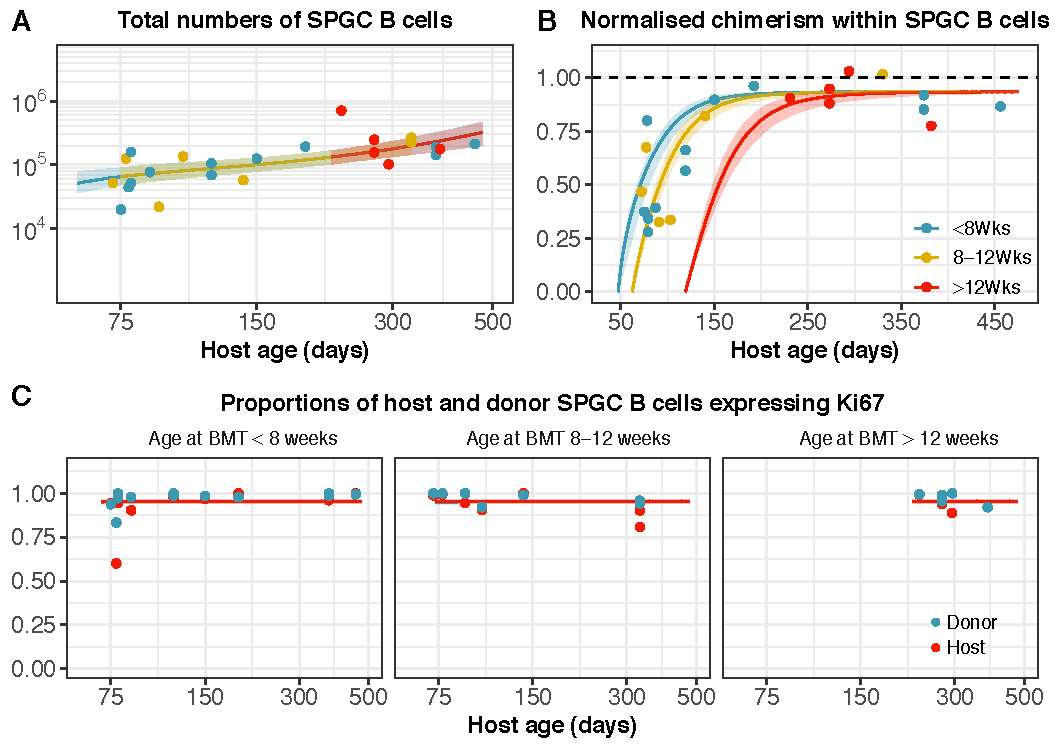
\includegraphics[scale = 0.85] {Results_SPGC_T2.pdf}}
		\caption{\textbf{Population dynamics of Spleen GC B cells in busulfan chimeric mice}, using the best-fitting model in which  cells divide at a constant rate, their mean lifespan increases with host age, and T2 B cells are their precursor population. Note that the chimerism normalised to T1 stabilises at a value <1,  equal to the chimerism in T2 normalised to T1. Solid lines denote the  best-fitting model predictions of the  timecourses  of (A) cell counts, (B) normalised chimerism  donor fractions and (C) \khi fractions. Prediction intervals (4.5$^{th}$ and 95.5$^{th}$ percentiles) were generated by drawing samples from the posterior distribution of parameter estimates. Different colours in (A) and (B) indicate mice grouped according to the age at BMT. Predictions for each group were drawn using the mean age at BMT within each group.}
		\label{fig:results_SPGC}
	\end{figure}
    
    
Using this information and, as before, fitting each model simultaneously to the numbers, chimerism and Ki67 expression levels of spleen GC B cells, we found that the model of time-varying loss with T2 B cells as their immediate precursor received strongest statistical support (Table~\ref{tab:GC-AICs}; fits shown in Fig.~\ref{fig:results_SPGC}).  We find that spleen GC B cells are far more dynamic than FM B cells,  with lifetimes and mean interdivision times of roughly half a day. The net effect of these processes yields a mean lifespan of spleen GC B cells of about 15 days in 7 week old mice (Table~\ref{tab:SPGC-parestm}). We infer that the expected lifespan of individual GC B cells doubles roughly every 8 months.
	%Models in which the rate of source influx or the inter-division time of GC cells varies with host-age produced poorer fits and received inferior statistical support  ({\looic} $\ge 8$).  
	We also infer that the maintenance of splenic GC B cell numbers is highly dependent on immigration, with approximately -- and remarkably -- 36\% of the population replaced by the cells from the circulatory T2 compartment every day.
	
		%: Table GC model weights
	\begin{table}[htbp]
		\begin{center}
			\renewcommand{\arraystretch}{1.25}
			\begin{tabular}{l l c c c c} 
				\toprule 
				&         & \multicolumn{4}{c}{\textbf{Model and {\looic}}} \\
				\cline{3-6}
				\textbf{Location} & Source     & {\small Simple homogeneous}&  {\small Time-dependent}    & {\small Kinetic heterogeneity} & {\small Incumbent} \\ 
				\toprule
				Spleen &   T1    &   17           &          9            &           33         &          12        \\ 
				     &   T2    &   10           &          0            &           33         &          9         \\ 
				     &   FM    &   13           &          8            &           32         &          9         \\ 
				\hline
				Lymph nodes &   T1    &   55           &          41           &           12         &          54        \\ 
				     &   T2    &   50           &          42           &           12         &          51        \\ 
				     &   FM    &   12           &          35           &           0          &          38        \\ 
				\hline
				\toprule 
			\end{tabular}
		\end{center}
		\caption{ \textbf{Comparison of models describing the population dynamics of Germinal center B cells in spleen and lymph nodes}. Model weights were calculated using the Leave-one-out information criterion (see Methods)} 
		\label{tab:GC-AICs}
	\end{table} 



	%The time-dependent model with T2 as the source has the fairly large probability (Akaike weight 94\%) to predict new information as compared to all the other models and sources explored in this analysis. 
	
% Table 2
\begin{table}[htbp]
\begin{center}
		\renewcommand{\arraystretch}{1.25}
		\begin{tabular}{l l }
			\toprule
			\textbf{Parameter}                                & \textbf{Estimates and 95\% CI} \\
			\toprule
			%Akaike weight (\% )                                     & 94                   \\
			Rate of influx from precursors ($\times 10^{-3}$ cells/day)      & 4.7 (3.2, 6.8)       \\
			Mean clonal lifespan  at age 7 weeks (days)   & 15 (13, 16)           \\
			Mean cell lifespan at age 7 weeks (days)             & 0.46 (0.34, 0.61)     \\			
			Mean inter-division time (days)                          & 0.48 (0.35, 0.64)     \\
			Time taken for $\tau$ to double(months)                  & 7.9 (4.5, 25)        \\
			Average time for {\khi} cells to transition to {\klo} (days)            & 5.2 (3.8, 6.7)  \\					
			\hline
			\toprule 
		\end{tabular}
	\end{center}
	\caption{ \textbf{Parameters governing homeostasis of GC B cells in the spleen}. Estimates from the best-fitting  model, in which thre longevity of splenic GC B cells increases with host age, and T2 cells are their direct precursor.  95\% credible intervals were estimated using the 2.5 and 97.5 percentiles of the posterior distributions of the parameter values.}
	\label{tab:SPGC-parestm}
\end{table} 
	
\subsection*{Lymph node GC B cells comprise a mixture of short-lived and persistent clones and likely derive from FM B cells}
As in the spleen, GC B cells in lymph nodes (LN) increase in numbers with age and donor and host cells express Ki67 at similar and high levels (Fig.~\ref{fig:results_LNGC}A and C). The numbers, chimerism and Ki67 expression of GC B cells in LN were best explained by a model invoking two subsets of cells with different kinetics, sourced by FM B cells (Fig.~\ref{fig:results_LNGC}).  This model was favoured with a weight of \red{XYZ\%} relative to all other models considered (Table~\ref{tab:GC-AICs}).

    \begin{figure}[htbp]
    	\centerline{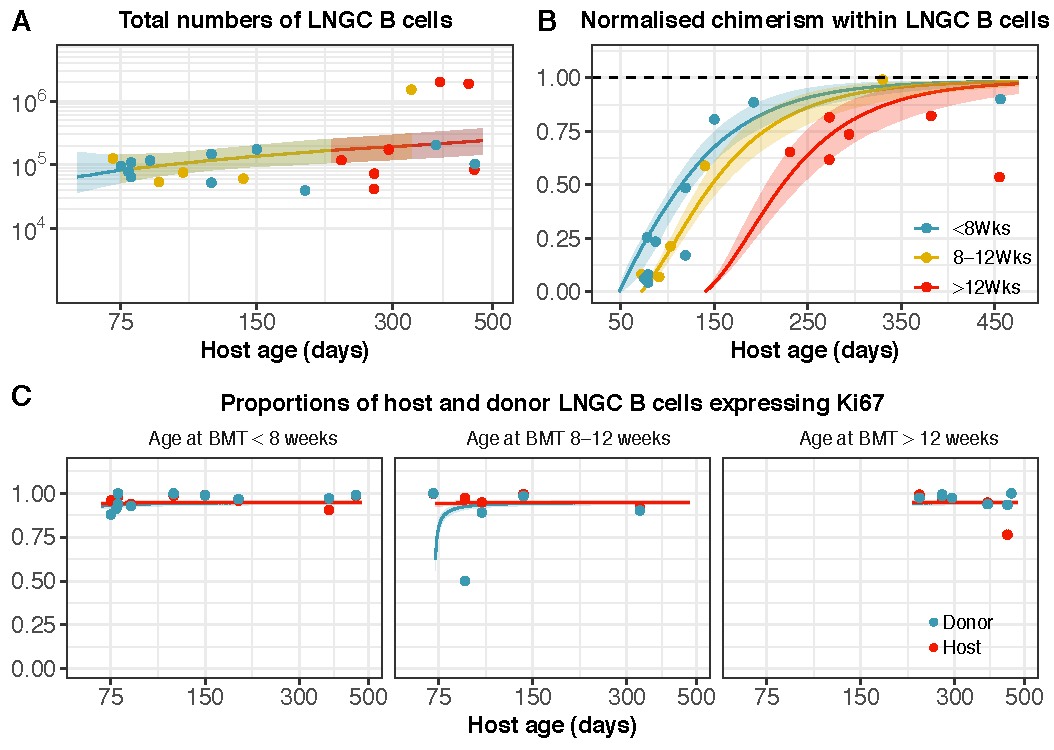
\includegraphics[scale = 0.85] {Results_LNGC_FM.pdf}}
    		\caption{ \textbf{Population dynamics of Lymph node GC B cells in busulfan chimeric mice}, using the best-fitting model of kinetic heterogeneity with FM B cells as the source. See Fig.~\ref{fig:results_SPGC} for details of fitting procedure.}
    		\label{fig:results_LNGC}
    \end{figure}
	
	
	


Our analysis reveals that some GC clones are  very short-lived, being lost from the lymph nodes within days (average clonal lifespan of $\sim$ 5 days, Table~\ref{tab:LNGC-parestm}) while others persist for on average 2 months (Table~\ref{tab:LNGC-parestm}).
%In this model the presence of pre-existing, persistent, host-derived  underlies the slow replacement kinetics of GC B cells in lymph nodes.
In a 7 week old mouse, we infer that the LN GC compartment contains short and long-lived clones in roughly equal proportions. We also find that roughly 25\% LN GC cells are replaced daily by new cells derived from the recirculating FM B cell pool.


%: Table 3
\begin{table}[htbp]
	\begin{center}
		\renewcommand{\arraystretch}{1.25}
		\begin{tabular}{l l l }
			\toprule
			\multirow{2}{*}\textbf{Parameter}                 & \multicolumn{2}{l}{\textbf{Estimates and 95\% CI}} \\
			                                                  & \small{Transient Subset}  & \small{Persistent Subset} \\
			\toprule
			%Akaike weight                                         &\multicolumn{2}{c}{99} \\         
			Rate of influx from precursors ($\times 10^{-2}$ cells/day)    & 7.0 (0.2, 40)        & 24 (12, 43)  \\
			Mean cell lifespan  (days)                            & 0.69 (0.42, 1.3)     & 0.90 (0.46, 1.9)  \\				
			Mean clonal lifespan (days)                            & 5.0 (1.2, 19)        & 68 (34, 130)  \\
			Mean inter-division time (days)                        & 0.91 (0.47, 2.0)     & 0.79 (0.46, 1.9)  \\
			Proportion of population at age 7 weeks         & 0.51 (0.17, 0.72)    & 0.49 (0.28, 0.83)    \\	
			Average time for {\khi} cells to transition to {\klo} (days)          & 5.1 (3.7, 6.6)       & 5.1 (3.7, 6.6)      \\	
			\hline
			\toprule 
		\end{tabular}
	\end{center}
	\caption{ \textbf{Parameter estimates for LN GC B cell homeostasis}, derived from the best-fit (kinetic heterogeneity) model with FM B cells as the precursor population.  Credible intervals were estimated by taking 2.5$^{th}$ and 97.5$^{th}$ percentiles of the posterior probability distribution of the parameter values obtained after fitting model to the data.}
	\label{tab:LNGC-parestm}
\end{table} 
	

    

\clearpage

	\subsection*{Discussion}
	\begin{itemize}
		\item GC cell dynamics vary between spleen and lymph nodes, as observed by slower replacement kinetics of LN GC cells  as compared to their splenic counterparts.
		Accordingly, our analysis predicts longer persistence of a large fraction of GC cells in lymph nodes than in spleen.
		
		\item Heterogeneity in LNGCs stems from pooling multiple LNs?
		
		\item Prolong GC reactions in response to viral antigens and gut microbes (Adachi et al. 2015, Bachman et al. 1996, Kasturi et al. 2011) may allow B cells to reach higher degree of affinity maturation $\rightarrow$ means to cope with constant antigenic drifts. 
		An important question is whether chronic GC response consists of long-lived GC cells or constant invasion of short lived cells maintaining a long-lived steady state?
		
		\item Ki67 in GC is result of active division and turnover and is not source derived. FM population has 10\% \khi cells while GC are $\sim$ 95\% \khi. 
	\end{itemize}
	

	
\section*{Methods}

%Specifically, the total numbers of FM B cells are given by
% 
% 
%	\be
%	\ddt{N_\text{FM}} = \;  \phi(t) + (\rho - \delta_{0}e^{-rt}) N_\text{FM},
%	\label{eq:FM_total}
%	\ee
%	
%	where $\phi(t)$ is the daily rate of influx from the source, whose kinetic was described  by fitting an empirical descriptor function to the timecourse of cell numbers. The size of the T1 and T2 populations  changed very little with host age and so these descriptor functions were nearly flat (\red{SHOW THIS IN SI/METHODS}). Time is measured from age 40 days, at which time the loss rate is $\delta_{0}$.
%	
%	
%	
	
	
\end{document}




